\documentclass[12pt]{article}
\usepackage{amsmath}
\usepackage{graphicx}
\usepackage{hyperref}
\usepackage[utf8]{inputenc}
\usepackage{geometry}
\usepackage{mathtools}
\usepackage{empheq}
\usepackage{listings}
\usepackage{xcolor}
\usepackage{caption}
\usepackage{subcaption}
\usepackage{setspace}
\usepackage{indentfirst}
\usepackage{authblk}
\usepackage{svg}

\graphicspath{ {./} }
\geometry{margin=1in}
\doublespacing
\captionsetup{labelfont=bf}

\title{CHEN 425 Workshop 1}
\author{Mark Levchenko}
\date{25 January 2023}

\begin{document}

% \maketitle

% \par\noindent\rule{\textwidth}{0.4pt}

\textbf{CHEN 425 ASPEN Simulation Report}

\textbf{Title:} Simulation of a Distillation Column Using the RADFRAC Model

\textbf{Workshop:} \#3

\textbf{Date:} February 15, 2023

\textbf{Prepared by:} Mark Levchenko

\textbf{To:} Professor Mahmoud El-Halwagi

\section{Summary of Results}

\subsection{Part 1}

The operating cost of the column based on the cost of heating and cooling the column is \$4,049,989/yr.

\subsection{Part 2}

Vapor profile:

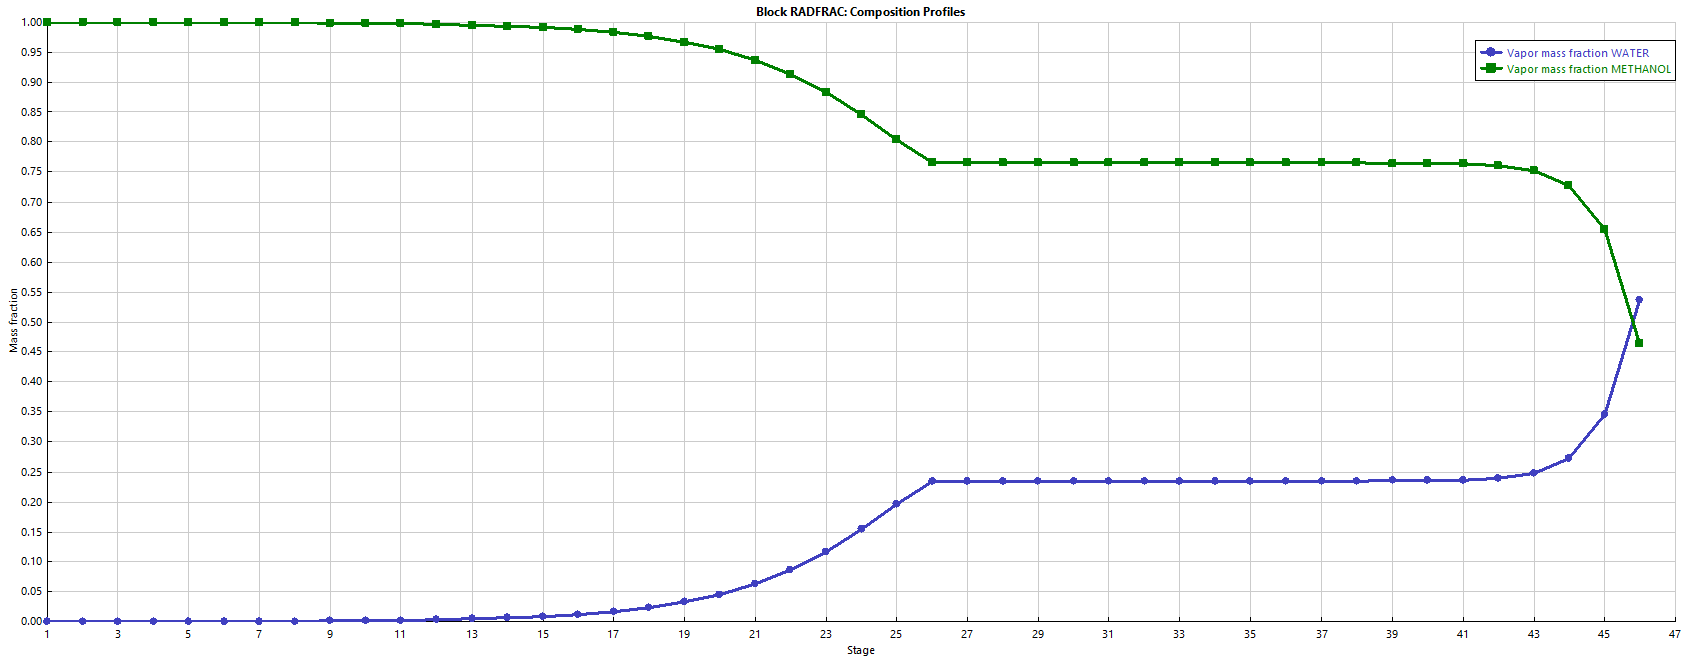
\includegraphics[scale=0.35]{vapi.png}

Liquid profile:

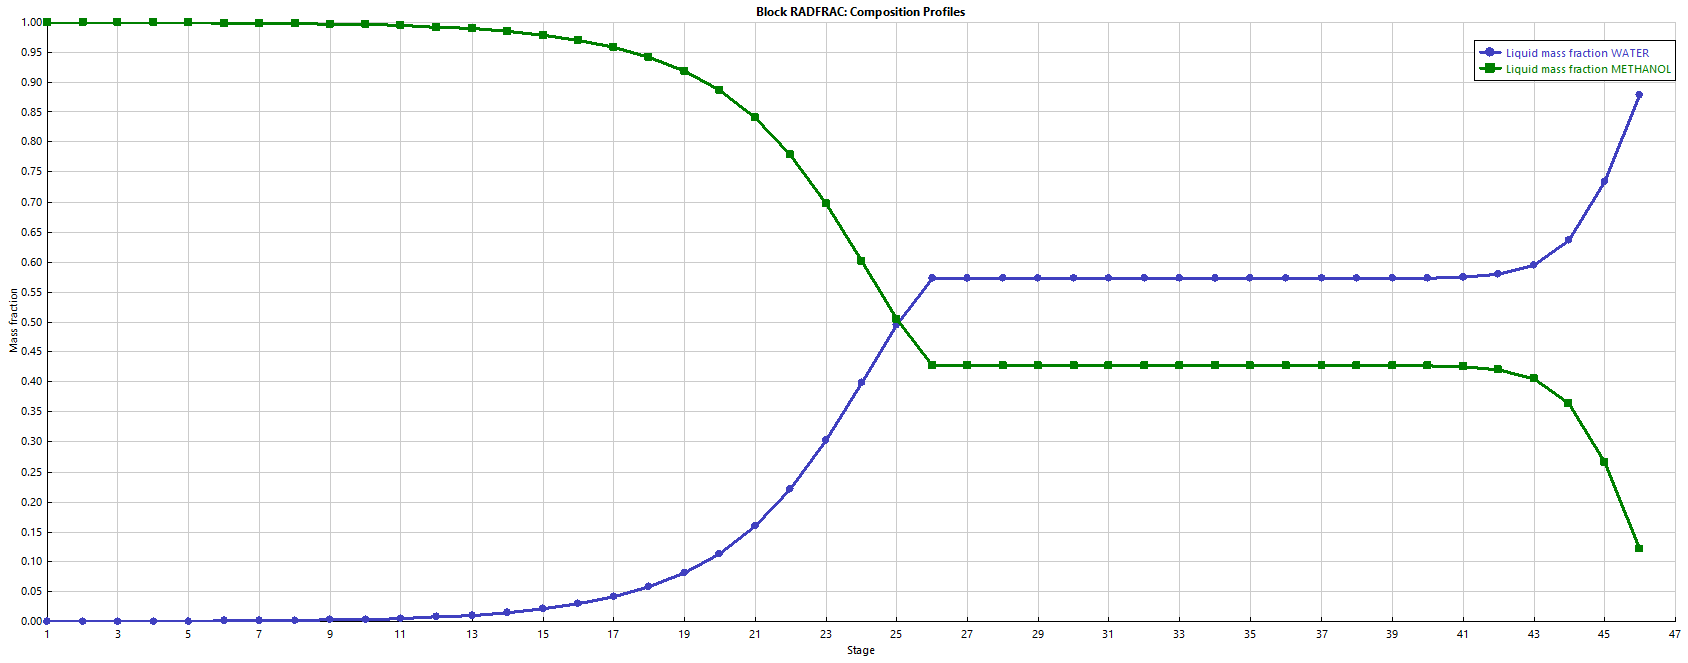
\includegraphics[scale=0.35]{liqi.png}

\subsection{Part 3}

The number of stages was reduced to 30, the feed stage was changed to 20, and the reflux ratio was reduced to 1.2.

Summary of column duties between base case and the case after changes were made to decrease operating costs:

\begin{tabular}{|c|c|c|}
    \hline
    Simulation & Heating duty (kW) & Cooling Duty (kW) \\
    \hline
    Base column & 15262.3 & 14833.4 \\
    With changes & 13938.2 & 13627.6 \\
    \hline
\end{tabular}



\section{Discussion of Simulation Results}

\subsection{Part 1}

The operating cost was calculated by finding the amount of steam and cooling water needed to heat and cool the column respectively. Heating and cooling duties were taken from the ASPEN simulation. Heating was achieved with the condensation of 683.56 kPa saturated steam. Cooling was achieved with liquid water with a heat capacity of 4.184 kJ/kg/$^\circ$C decreasing in temperature 20$^\circ$C.

\textbf{Table 2.14} in the textbook contains costs for various utilities. From this table, a steam cost of \$15/ton and a cooling water cost of \$0.10/m$^3$ were used in the operating cost calculations. Conservatively, the highest prices of each range were taken as the basis for the operating cost calculations.

Operating cost calculation:

\begin{align*}
    Q_{\mathrm{cooling}} &= 14833.4 \text{ kW} \\
    C_P &= 4.184 \text{kJ/kg/$^\circ$C} \\
    \Delta T &= 20 \text{$^\circ$C} \\
    \intertext{Cost of cooling water is \$0.10/m$^3$}
    \intertext{Operate 31536000 s/yr}
    \text{Cooling cost} &= \frac{14833.4 \text{ kW}}{4.184 \text{kJ/kg/$^\circ$C} \cdot 20 \text{$^\circ$C}} \cdot \frac{1 \text{ m}^3}{1000 \text{ kg}} \cdot 31536000 \text{ s/yr} \cdot \$0.10/\mathrm{m}^3 \\
    \text{Cooling cost} &= \$559017\text{/yr} \\
    Q_{\mathrm{heating}} &= 15262.3 \text{ kW} \\
    \Delta h_v &= 2068.1 \text{kJ/kg}
    \intertext{Take the cost of 683.56 kPa steam as \$15/ton}
    \text{Heating cost} &= \frac{15262.3 \text{ kW}}{2068.1 \text{kJ/kg}} \cdot \frac{1 \text{ ton}}{1000 \text{ kg}} \cdot 31536000 \text{ s/yr} \cdot \$15/\mathrm{ton} \\
    \text{Heating cost} &= \$3490971\text{/yr} \\
    \mathrm{OPEX} &= \$4,049,989\text{/yr}
\end{align*}

\subsection{Part 2}

From stage 27 to stage 42, the vapor and liquid compositions do not change. The lack of change suggests that these stages may not be necessary to achieve a sufficient purity of products.

\subsection{Part 3}

The Total duty decreased approximately 8.4\%. The decrease will result in approximate savings of \$340,000\text{/yr}. 

From Part 2, there is a section of the column where the vapor and liquid compositions do not change. Removing these stages has little effect on the product purity because these stages were not doing anything to begin with. Removing them will decrease the capital and installation costs due to the smaller column size.

Lowering the reflux ratio lowers the amount of liquid in the column which reduces the amount of heat necessary to vaporize the liquid in the column. Lowering the reflux ratio had the biggest impact on column operating costs because it directly decreases the amount of heating and cooling necessary.

\section{Simulation Screenshots}

Main flowsheet:

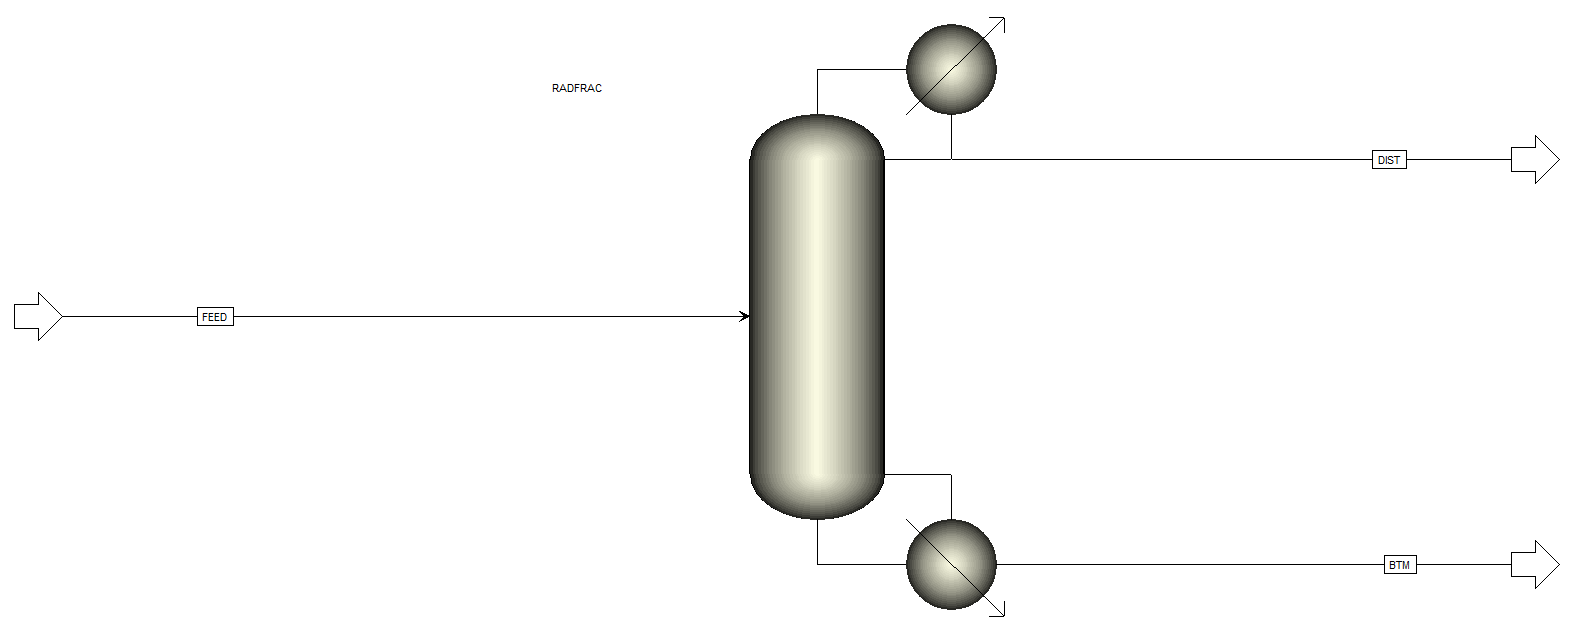
\includegraphics[scale=0.3]{flowsheet.png}

\subsection{Part 1}

RADFRAC results for part 1:

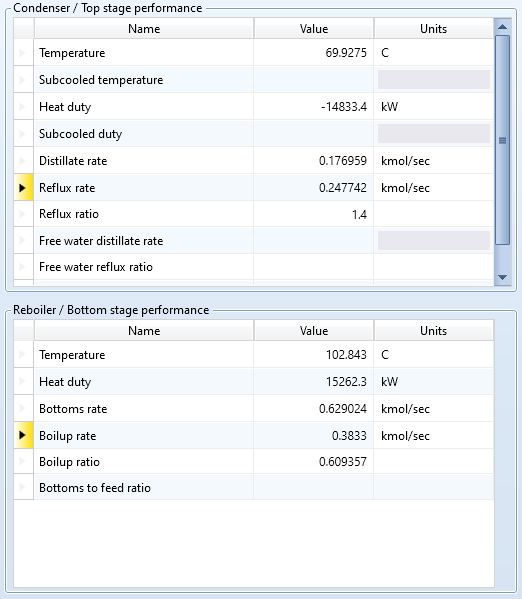
\includegraphics[scale=1]{parti.png}

\subsection{Part 2}

Profile plots are in the summary of results section for part 2.

\subsection{Part 3}

RADFRAC results with reduced reflux ratio and stages:

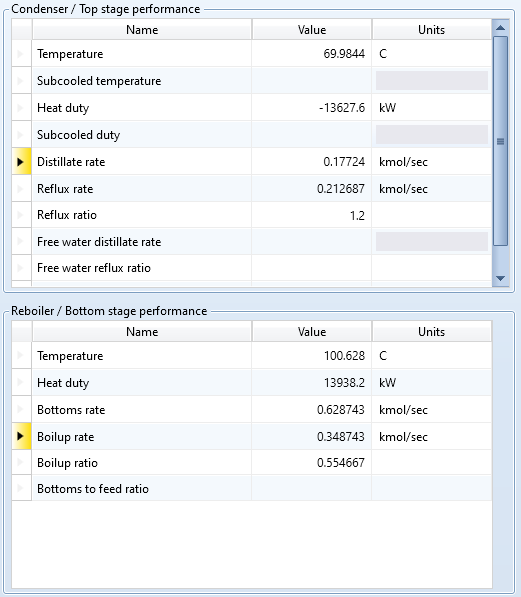
\includegraphics{part3.png}

Purity of distillate is still 99\%.

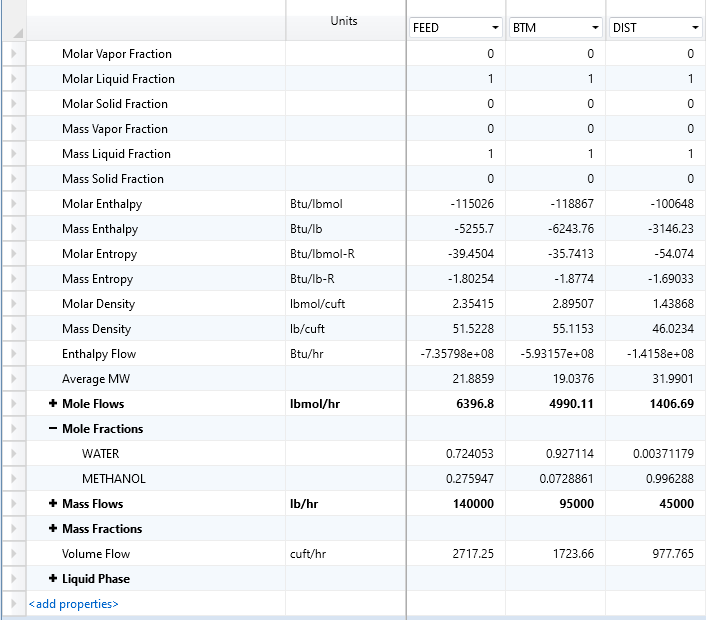
\includegraphics[scale=0.8]{stream3.png}



\section{Conclusions}

The cost of cooling and heating a distillation column is significant. \$4,000,000 per year in operating costs outweighs any capital costs or any other costs associated with the operation of the column like electricity.

The initial design of the column included too many stages. The composition profiles demonstrated that the additional stages of the initial design were not doing anything to improve the separation. To reduce the capital costs, these stages were removed, and the purity of methanol did not decrease significantly. Furthermore, the operating cost of the column could be decreased by more than 8\% by decreasing the reflux ratio to 1.2.


\end{document}